%\documentclass[twoside, a4paper,12pt]{scrartcl} % For two-sided printing on paper.
\documentclass[oneside, a4paper,12pt]{scrartcl} % For one-sided printing or screen.


% ---------------------------------------------------
% General
% ---------------------------------------------------
\usepackage{graphicx} % For including figure
\usepackage[english]{babel} % Set default language for things like "Figure" or "References"
\usepackage{url} % For typesetting URLs

% additionally useful--------------------------------
\usepackage{seqsplit} % for automatic line breaks 
\usepackage{lscape} % enable landscape format 

% ---------------------------------------------------
% Fonts and typesetting
% ---------------------------------------------------
\usepackage[utf8]{inputenc} 
\usepackage[T1]{fontenc} 
\usepackage{gensymb} % symbols for e.g. formulas 

% ...............
% Load serif font 
% ...............
%\usepackage[rm]{libertine} % Another favorite of mine: font designed for Linux OS.
\usepackage{lmodern} % Classic Latex font - easy to recognize as Latex document.

% ...............
% Load sans-serif font
% ...............
% Just an aesthetic choice, if you do not like the computer-modern-sans-serif
%\usepackage{helvet} % Classic font, you can't go wrong with this.
\usepackage{roboto} % Font designed for webpages by Google.
%\renewcommand*\familydefault{\sfdefault} % activate if all text should be sans serif

% ...............
% Load typewriter font. Useful for \verb|text| environment.
% ...............
\renewcommand*\ttdefault{cmvtt} 


% ---------------------------------------------------
% Typesetting and layout
% ---------------------------------------------------
\linespread{1.15} % Slightly increased line spacing.


\usepackage[activate={true,nocompatibility},final,tracking=true,kerning=true,spacing=true,factor=1100,stretch=10,shrink=10]{microtype}
% activate={true,nocompatibility} - activate protrusion and expansion
% final - enable microtype; use "draft" to disable
% tracking=true, kerning=true, spacing=true - activate these techniques
% factor=1100 - add 10% to the protrusion amount (default is 1000)
% stretch=10, shrink=10 - reduce stretchability/shrinkability (default is 20/20)


% Use this to manipulate the page margin width.
\usepackage[a4paper,top=2.5cm,left=2.5cm,right=2.5cm,bottom=2.7cm]{geometry}


% This gives the figure captions a more professional look.
\usepackage[margin=24pt,format=plain,font=footnotesize,labelfont=bf,skip=10pt]{caption}  

% Alternate figure caption setup:
% \usepackage[capposition=top]{floatrow} 
% Caption of figure is moved to the top, leaving space for a note below the figure. 
% Enable line 53 - 59 in the content script to see an example.


% This gives the abstract a more professional look.
\usepackage{abstract}
\renewcommand{\abstractnamefont}{\normalfont\bfseries} % Set the "Abstract" text to bold
\renewcommand{\abstracttextfont}{\small} % Set the abstract itself to small italic text


% Indentation and extra spacing for paragraphs
\setlength{\parindent}{8pt}


%\usepackage{indentfirst} % without this, the first paragraph of a section is NOT indented.
\setlength{\parskip}{4pt plus 2pt minus 1pt}

% For persistent issues with overfull boxes, use with caution!
%\setlength{\emergencystretch}{5pt}  % when enabled, this allows a slightly larger tolerance in paragraphs with overfull boxes without changing the overall tolerance

% ---------------------------------------------------
% Important and useful packages
% ---------------------------------------------------
% If you want a figure to include more than a single image file. Not terribly important, but I use it in this sample file.
\usepackage{subcaption}

\usepackage{csquotes} % proper typesetting of quotes
\usepackage{soul} % strike out and underline letters
\usepackage{color}

% Optional, if you want linenumbers in the margin in the pdf. 
% Can be useful for proofreading. Switch on with "\linenumbers" in the text.
\usepackage{lineno} 

% Optional for draft manuscripts: put all figures at the end of the document
% and put a "Figure X around here" placeholder in the text.
%\usepackage[nolists]{endfloat}

% For typesetting epigraphs at chapter beginnings.
\usepackage{epigraph}
\renewcommand{\epigraphsize}{\small}
\setlength{\epigraphwidth}{0.4\textwidth}

% For typesetting of authors and affiliations on title page for articles.
% Not necessary for thesis title page.
\usepackage{authblk}
\renewcommand\Authfont{\normalsize}
\renewcommand\Affilfont{\small\itshape}

% For Figures embedded in text.
\usepackage{wrapfig}

% Nice options for tables.
\usepackage{multirow}
\usepackage{booktabs}
\setlength\tabcolsep{8pt}

% Adds some additional options for including figures. 
\usepackage{graphicx}


% ---------------------------------------------------
% Bibliography
% ---------------------------------------------------
\usepackage{natbib}
\renewcommand{\bibfont}{\small} % Make the font size smaller for the bibliography
\usepackage[numbib]{tocbibind} % This makes the Bibliography a numbered section.
%\addto{\captionsenglish}{\renewcommand{\bibname}{References}} % use this to rename the Bibliography to "References"

% ---------------------------------------------------
% Headers and footers
% ---------------------------------------------------
\usepackage[headsepline]{scrlayer-scrpage} % scrpage2 deprecated 
\clearpairofpagestyles %clearscrheadfoot deprecated
\pagestyle{scrheadings}
\automark{section}
\ohead{\pagemark}
\chead{}
\ihead{\headmark}


% ---------------------------------------------------
% Text shortcuts
% ---------------------------------------------------
\usepackage{xspace} % optional white space if not followed by punctuation.
\newcommand{\fc}{flux capacitor\xspace}
\newcommand{\roc}{receiver operating characteristic\xspace}



% ---------------------------------------------------
% To do notes in page margins
% ---------------------------------------------------
\usepackage[x11names]{xcolor}
\usepackage[colorinlistoftodos, textsize=footnotesize, linecolor=red!60, backgroundcolor=Ivory2, bordercolor=red!60]{todonotes}
\reversemarginpar



% -----------------------------------------------------------------
% Main text.
% -----------------------------------------------------------------
\begin{document}
	

% ---------------------------------------------------
% Title section
% ---------------------------------------------------
\begin{titlepage}
	\titlehead{
\includegraphics[width=8cm]{Figures/WWU_Logo1_PantoneBlack7}\\
		~\\
		Westfälische Wilhelms-Universität Münster\\
		Institut für Psychologie\\
		Abteilung für Allgemeine Psychologie\\
		AE Busch}
	
	\subject{\vspace*{1.5cm}Masterarbeit im Studiengang Psychologie}
	
	\title{\vspace*{1cm} Verbessert Kaffeetrinken das Kurzzeitgedächtnis?}
	
	\subtitle{Hier kann ein Untertitel stehen, falls es sich anbietet\vspace*{2cm}}
	\author{Karla-Heinz X. Irgendwer\\
		Matrikelnummer: 4711-0815}
	\date{\today}
		\publishers{\vspace*{3cm} \begin{flushleft}
				1. Gutachter: Prof. Ahfrau\\ 2. Gutachter: Prof. Behmann
			\end{flushleft}} 
		
	\dedication{}
\end{titlepage}	
\maketitle

\tableofcontents
\newpage

% Optional: switch on line numbering in pdf.
% \linenumbers

%\include{Content} %  \include{file} starts on a new page.


\begin{abstract} 
This is the abstract, in which we describe why this study is awesome. It's tremendous! Honestly folks, don't trust what the dishonest media say about this study. It is terrific, believe me. 
\end{abstract}  

%\newpage

\section{Introduction}

\epigraph{\textit{
	If you end up with a boring miserable life because you listened to your mom, your dad, your teacher, your priest, or some guy on television telling you how to do your shit, then you deserve it!}}
	{Frank Zappa}

\subsection{Sectioning commands}
\subsubsection[short title for toc]{Even lower-level section with a really, really, long title. Boy, is this a long title!}
\paragraph{This is a paragraph}

\LaTeX will typeset your headlines properly and even count and index them automatically if you use these envirnoments: \verb+\section{}+, \verb+\subsection{}+, \verb+\subsubsection{}+, and \verb+\paragraph{}+. If you want an unnumered section, use the starred version: \verb+\section*{}+



\subsection{Text formatting}
Some \LaTeX-specific formatting tips are provided here. Proper quotation marks are done ``this way'' or \enquote{this way}. 

To add emphasis, words should be in \textit{italics}, not \textbf{bold} or \underline{underlined}. Certainly not \st{strike through}!

A line break requires an empty line between two lines of text in your code. Do not use \verb+\newline+ to force a new paragraph.

There is a difference between three types of dashes: (1) simple dash for composite words such as Latex-specific; (2) double dash for numerical ranges such as 2013--2014; (3) long dashes---I am sure you have seen them before---for included sentences.

There should be a non-separable white space between numbers and their units of measurement: my hat size is 58~cm; not: 58cm. not: 58\newline cm.

\todo[inline]{This is a longer note-to-self kind of text. I describe what I think. Maybe I need to work on this section more. Or delete it? Maybe I just ask my cat what to do with it.}



\subsection{Text shortcuts}
If you use bits of text again and again, make your life easier with
\newline
 \verb+ \newcommand{\blabla}{my little shortcut}+. This turns a long string of text into a tiny little shortcut. I use my \fc a lot, every day a new \fc. Everybody loves the \fc and the \roc! I repeat: \roc, \roc, \roc!

\begin{figure}[t]
	\centering
	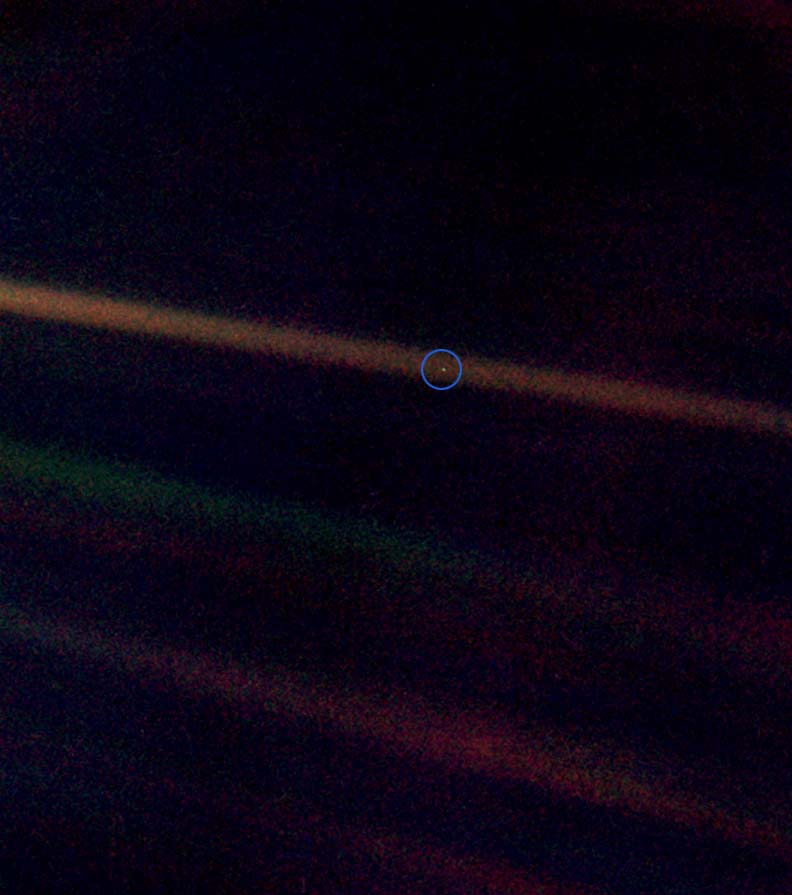
\includegraphics[width=0.25\linewidth]{Figures/PaleBlueDot.jpg}
	\caption{A pale, blue dot, suspended in a sunbeam \citep{NASA}.}
	\label{samplefig}
\end{figure}

% Example for alternate figure caption setup that allows for notes below the figure. Requires line 65 in the template. 
%\begin{figure}[t]
%	\centering
%	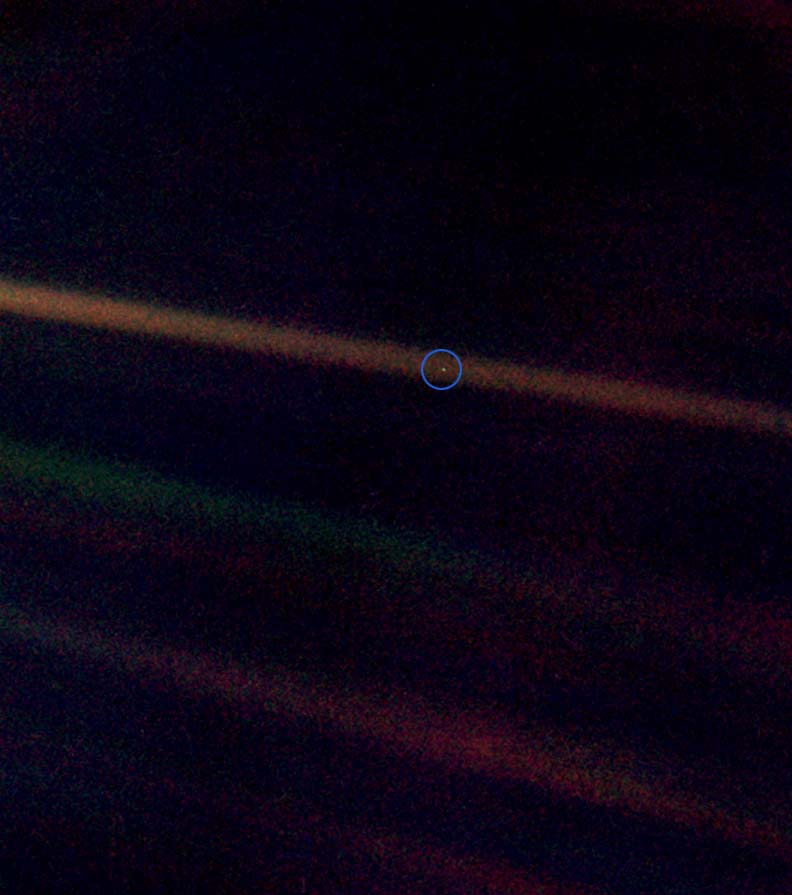
\includegraphics[width=0.25\linewidth]{Figures/PaleBlueDot.jpg}
%	\caption{A pale, blue dot, suspended in a sunbeam \citep{NASA}.}
%	\floatfoot{\textit{Note.} Blue Dot marks spaceship location.}
%	\label{samplefig}
%\end{figure}

\subsection{Environments}

Bullet point environments:
\begin{itemize}
\item In New York;
\item Rio;
\item Tokyo.
\end{itemize}

Enumerated environments:
\begin{enumerate}
\item Stop science funding;
\item Call Wladimir;
\item Build wall.
\end{enumerate}

\subsection{Within-paper references and figures}
\label{withpaperrefs}

You can easily refer to sections within the paper. This is explained in section \ref{withpaperrefs}. You can also refer to figures. The numbering is done fully automatically, see Figure \ref{samplefig} on page \pageref{samplefig}. Note that figures in vector format (.eps; .pdf) are preferred over bitmap formats (.jpg). Figure \ref{pdf_vs_jpg} illustrates why vector formats are better than bitmaps.

We can also use footnotes; little annotations that appear at the bottom of the page\footnotemark.

\footnotetext{This is the footnote text.}

\newpage

\paragraph{Figures embedded in text.}

\begin{wrapfigure}{r}{6cm}
    \centering
    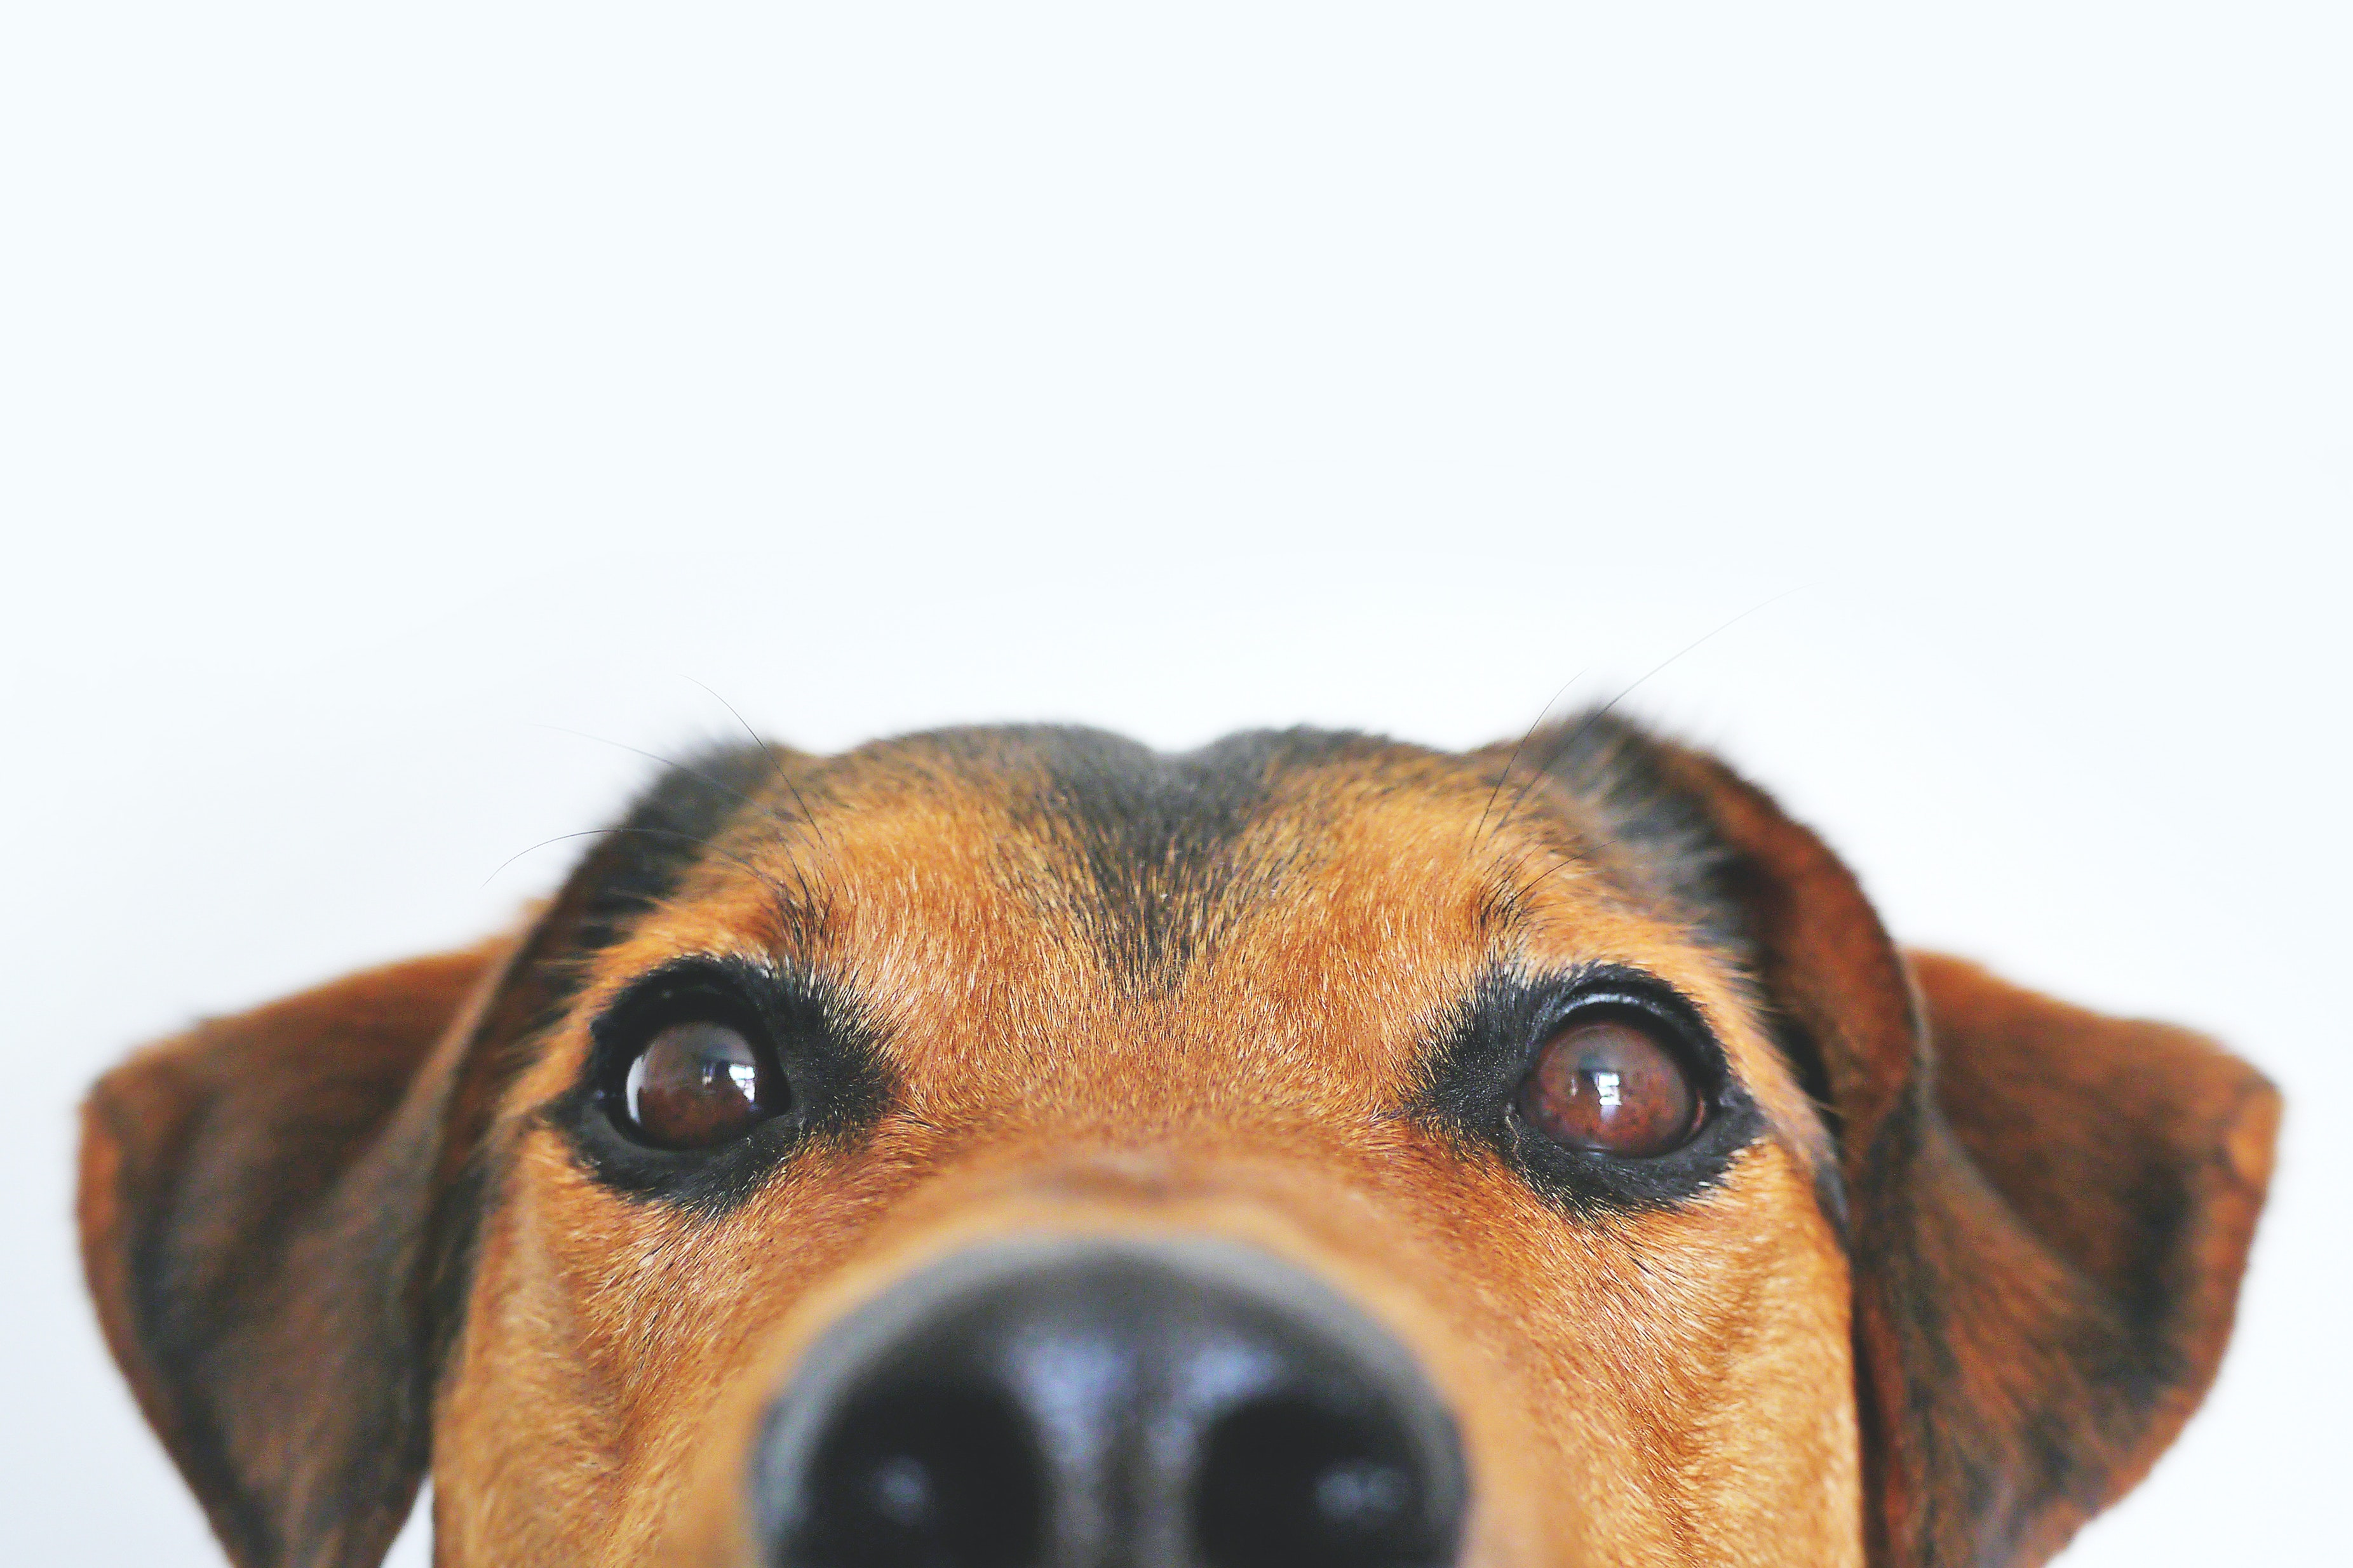
\includegraphics[width=0.8\linewidth]{Figures/dog.jpg}
	\caption{A very good boy.}
	\label{dog}
\end{wrapfigure}

Figures are usually scaled full size and isolated from text. In some instances, providing a small picture right next to what you are describing can be useful for a reader. Let's use this cute dog as an example: I have added it as a \textit{wrapfigure} right next to this paragraph. Now you can directly enjoy a visual of this very good boy while reading about his floppy brown ears and smart nose!


\subsection{Formulas}
There are two possibilities for typesetting a formula in \LaTeX. Simply using \verb+$+ signs inserts it \textit{inline} like this:  $\alpha + \beta + \gamma = 180\degree$. If the formula is not part of your paragraph or you would prefer to typeset it in its own line, use the following \textit{display} mode:

\begin{displaymath}
x_{1,2} = \frac{-b \pm \sqrt{b^2-4ac}}{2ac} 
\end{displaymath}

In a section containing multiple formulas you can also use \verb+{equation}+ instead of \verb+{displaymath}+ to automatically number the equations for easier referencing.

\begin{equation}
A = \frac{1}{2} \pi r^2
\end{equation}

Let's add a second formula here:

\begin{equation}
E = mc^2
\end{equation}

For the appropriate \LaTeX code for specific symbols not displayed in this example see comprehensive lists, e.g. \url{https://oeis.org/wiki/List_of_LaTeX_mathematical_symbols}.

\subsection{Tables}

Setting tables in \LaTeX can be tricky, especially if you want to connect certain cells. Use the commands \verb+ \multicolumn{x}{c}{"columns header"}+ to connect x columns and \verb+ \multirow{y}{*}{"rows header"}+ to connect y rows - nest as required. A minimal example:

\begin{table}[h!]
    \centering
    \caption{The use of multicolumns and - rows.}
    \label{ex_table}
    \begin{tabular}{@{}l*{5}{c}@{}} 
    \toprule
    column a & \multicolumn{2}{c}{multicolumn b + c} & \multicolumn{2}{c}{multicolumn d + e}\\
    \midrule
    \addlinespace
    \multirow{2}{*}{multirow 1 + 2 }
    & \multicolumn{2}{c}{cell 1} & {cell 2} & {cell 3}\\ 
    & {cell 4} & {cell 4} & {cell 6} & {cell 7}\\ 
    \bottomrule
    \end{tabular}
\end{table}

% using booktabs commands like \toprule or \bottomrule creates nicer lines than \hline & co.!

Reference tables like Table \ref{ex_table} on page \pageref{ex_table} as explained for figures in section \ref{withpaperrefs}.


\subsection{Citing literature}

We can refer to papers directly. I greatly admire the study by \cite{ADRIAN1934}. We can also cite papers in parenthesis \citep{ADRIAN1934}. Sometimes, we want to write something additionally into the parentheses \citep[the study by][is also not bad]{Allard2011}. For all details on different ways to cite literature with the natbib package, refer to \url{http://merkel.texture.rocks/Latex/natbib.php}. 

We can also typeset quotes nicely:

\begin{displayquote}
The aggregate of all our joys and sufferings, thousands of confident religions, ideologies and economic doctrines, every hunter and forager, every hero and coward, every creator and destroyer of civilizations, every king and peasant, every young couple in love, every hopeful child, every mother and father, every inventor and explorer, every teacher of morals, every corrupt politician, every superstar, every supreme leader, every saint and sinner in the history of our species, lived there---on a mote of dust, suspended in a sunbeam \citep[][S. 6--7; see Figure \ref{samplefig}]{Sagan1994}.
\end{displayquote}


\todo[]{Anything else I should mention here?}




\begin{figure}[t]
	\centering
	
	\begin{subfigure}[t]{0.45\textwidth}
		\centering
		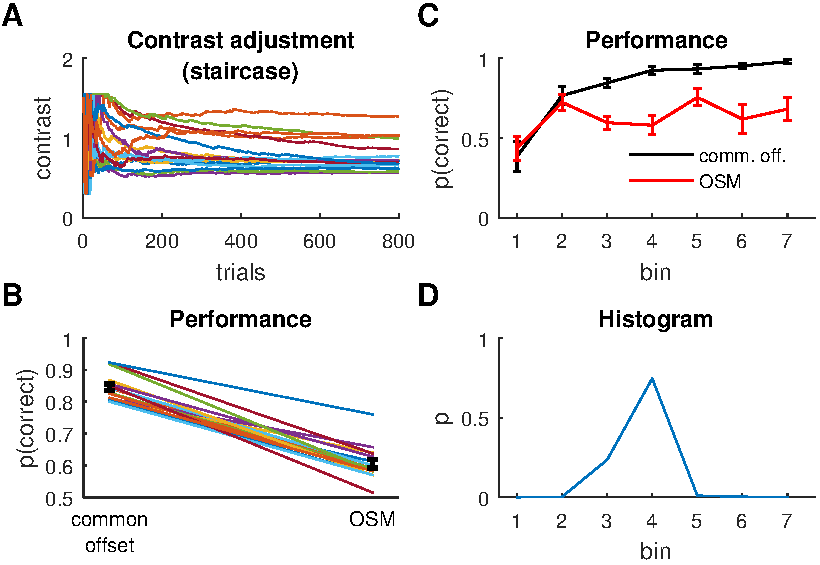
\includegraphics[width=\linewidth]{Figures/Resultspdf} 
	\end{subfigure}		
	\hfill % If you want to place the figures side by side there should be no empty line between subfigures.		
	\begin{subfigure}[t]{0.45\textwidth}
		\centering
		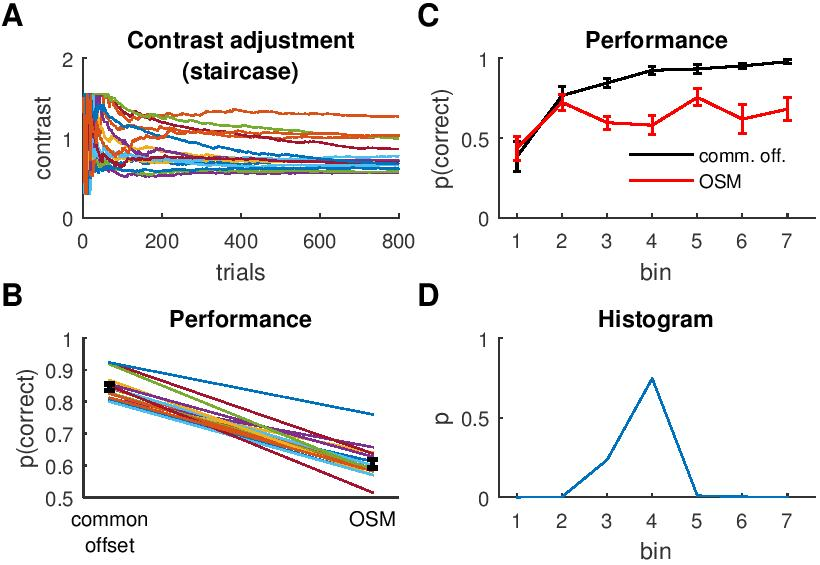
\includegraphics[width=\linewidth]{Figures/Resultsjpg} 
	\end{subfigure}
	
	
	\caption{Comparison of vector format and bitmap format. Left: figure built from a *.pdf file. The separate lines are easy to see, can be zoomed in and text is searcheable in the pdf output. Right: figure built from *.jpg. Doesn't look so good.}
	\label{pdf_vs_jpg}
\end{figure}

 % \input{file} does not start on a new page.


\bibliographystyle{apalike}
\bibliography{bibliography}

\end{document}
